\scanpage{171}\mspage{26}%
this to suppose that $X$ is ``locally homotopically trivial'', which ensures that the pro-simplicial set that Artin-Mazur associate to it (by the procedure of nerves of 'hypercoverings) is essentially constant in the ordinary homotopy category - thus $X$ defines a usual homotopy type. This is \uline{not} the case of course for the étale topos of a scheme, For such a case, the fundamental $n$-groupoid must be conceived as a \uuline{pro}-$n$-groupoid (nothing surprising in that, given the familiar theory \unsure{of the|of the} $\pi_1$) ; and $\unsure{\mathcal E|E}_n$ as an $(\mathrm{ind})$-$n$-category (\unsure{the|the} ind-structure corresponding to the requirement of local triviality, for a varying $n$-stack, with respect to finer and finer coverings of $X$).

\figure{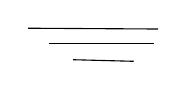
\begin{tikzpicture}[x=1cm,y=1cm]
\draw (0,0)--(1.65,-.01);
\draw (.27,-.19)--(1.60,-.19);
\draw (.57,-.40)--(1.34,-.42);
\end{tikzpicture}}

I understand however your instinctive resistance to conceiving this extreme stripping down of a beautiful topos $X$, to the point of%
% Isolated short pen stroke at the right edge, between manuscript baselines 21 and 22; no textual interpretation.
\margin{\figure{\begin{tikzpicture}[x=1cm,y=1cm]\draw[line width=.5pt] (0,0)--(.14,.025);\end{tikzpicture}}}
retaining only its meagre homotopy type. What is more, I am convinced that in%
% Isolated small black point at the lower right, below and right of the final n; origin uncertain, not assigned sentence punctuation.
\margin{\figure{\begin{tikzpicture}[x=1cm,y=1cm]\fill (0,0) circle[radius=.018];\end{tikzpicture}}}
% archive sheet number: 171
